\documentclass[a4paper,12pt]{article}
\usepackage[english]{babel}
\usepackage[utf8]{inputenc}

%
% For alternative styles, see the biblatex manual:
% http://mirrors.ctan.org/macros/latex/contrib/biblatex/doc/biblatex.pdf
%
% The 'verbose' family of styles produces full citations in footnotes, 
% with and a variety of options for ibidem abbreviations.
%
\usepackage{graphicx}
\usepackage{csquotes}
\usepackage[style=verbose-ibid,backend=bibtex]{biblatex}
\bibliography{sample}

\usepackage{lipsum} % for dummy text

\title{An analysis of model-based Interval Estimation for Markov Decision Processes}

\author{Shayan Amani}

\date{\today}

\begin{document}
\maketitle

\section{Summary}
This paper discusses Model Based Interval Estimation approach in detail and then it tries to demonstrate benefits of using another version of the mentioned method which it introduces a new metric (more specifically an "online" metric) to the problem. Then the authors demonstrate that the proposed method works even in worst case scenario. Model Based Interval Estimation with exploratory bonus or shortly MBI-EB which is the proposed approach by the authors has been proved that is PAC so it takes advantage of time guarantee to reach the  admissible accuracy. As it goes further, they have gone through proofs of the theorems that they framed out but the case that they have tried to experiment their method is not clearly explained.


% 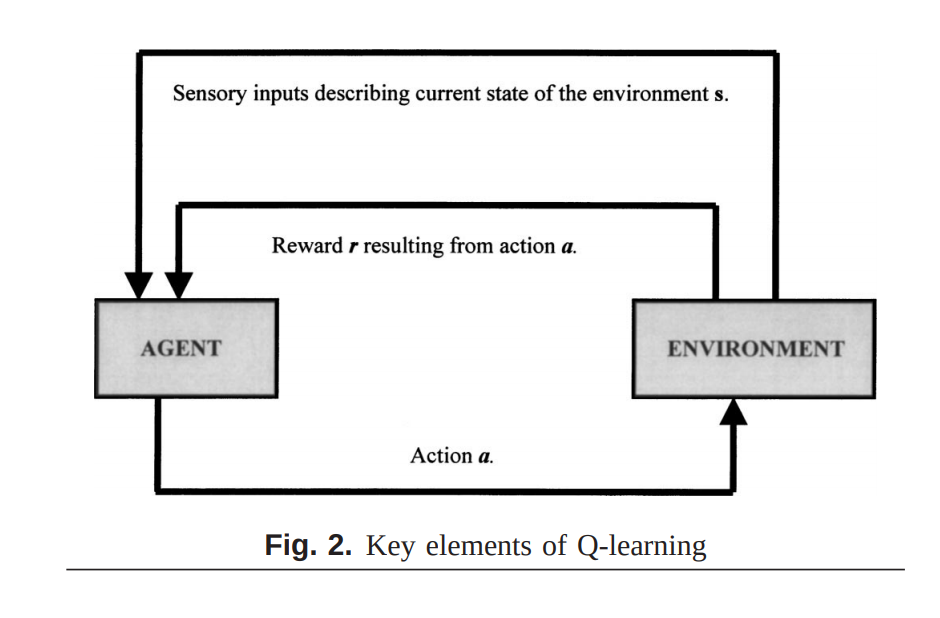
\includegraphics[width=1\columnwidth]{elements.png}




% This is an example citation \autocite{ginsberg}.
% \lipsum[1] % dummy text

% This is another example citation \autocite{brassard}.
% \lipsum[2] % dummy text

% This is a repeated citation \autocite{brassard}.
% \lipsum[3] % dummy text

% This is another example citation \autocite{adorf}.
% \lipsum[4] % dummy text 

\end{document}